\documentclass{article}

\usepackage[preprint]{neurips_2026}
\usepackage[utf8]{inputenc}
\usepackage[T1]{fontenc}
\usepackage{hyperref}
\usepackage{url}
\usepackage{booktabs}
\usepackage{amsfonts}
\usepackage{amsmath}
\usepackage{nicefrac}
\usepackage{microtype}
\usepackage{graphicx}
\usepackage{multirow}
\usepackage{xcolor}

\newcommand{\omini}{\texttt{o4-mini}}

\title{Harder Instances, Higher Accuracy:\\Difficulty, Oracles, and Item Dependence in\\LLM Robustness Benchmarks}

\author{%
  Anonymous Author(s)\\
  Affiliation\\
  Address\\
  \texttt{email}
}

\begin{document}

\maketitle

\begin{abstract}
Benchmarks that perturb the surface form of reasoning problems report accuracy drops and
attribute them to memorisation. We audit what those drops measure. Applying six surface
variants to 219 problems across arithmetic, planning, and algorithmic optimisation, on six
models, we find that three confounds each independently produce drop-shaped signals. First,
the answer-checker is itself a program: because obfuscation perturbs exactly the tokens a
checker parses, oracle failure is correlated with the treatment rather than random, and it
biases toward the memorisation hypothesis. Correcting one such defect moves a single cell
from $0.043$ to $0.252$ with zero movement on the unperturbed condition. Second, canonical
and regenerated instances are not difficulty-matched. On Blocksworld, regenerated instances
are harder on every structural measure we can compute, including optimal plan length from an
admissible planner, yet four of six models score \emph{higher} on them; Claude Sonnet~4 moves
from $0.170$ to $0.638$. $n$-gram proximity to public corpora does not account for this gap.
Third, benchmark items are not independent: our algorithmic bank of 110 problems collapses to
51 clone families, so nominal intervals are $1.6$--$2.7\times$ too narrow. Beyond the
confounds, two structural results survive. Surface fragility has no item-level locus --- no
problem fails across all models in arithmetic or algorithms --- and plan-execution consistency
does not predict rename survival ($r{=}0.156$, $p{=}0.060$), so robustness is not a single
construct. We release per-instance verifier logs and a gold-in-gold-out harness that detects
oracle failure before it reaches a results table.
\end{abstract}

\section{Introduction}

A now-standard evaluation protocol takes a reasoning benchmark, perturbs the surface form of
each item while preserving its solution, and reports the accuracy drop as evidence that models
rely on memorised surface patterns rather than generalisable procedure
\citep{mirzadeh2025gsmsymbolic, valmeekam2023planbench, wang2024rupbench, huang2025mathperturb}.
The inference is attractive because the manipulation is clean: if the problem is logically
identical and only the words changed, a drop looks like direct evidence about representation.

This paper asks what else could produce that drop. We are not arguing the phenomenon is
absent. We are arguing that the standard protocol, as implemented across several widely-used
benchmarks including our own first implementation, admits at least three alternative
explanations that are rarely controlled and that each bias in the same direction as the
hypothesis under test.

\paragraph{The oracle is a program.} Automated evaluation depends on an answer-checker, and in
software testing the reliability of that checker is known as the \emph{test oracle problem}
\citep{barr2015oracle}. Obfuscation benchmarks have an unusually severe version of it. The
perturbation renames exactly the entities, actions, and identifiers that a checker must parse
to score an answer. A checker that silently fails to invert the rename returns
\texttt{incorrect} on the perturbed condition and \texttt{correct} on the canonical one, for
every model. This is not measurement noise: the failure is correlated with the treatment, so
it produces bias, and the bias points toward the memorisation hypothesis. We document three
such defects in our own pipeline (Section~\ref{sec:oracle}), all of which moved accuracy
upward on the perturbed condition once repaired.

\paragraph{Regenerated instances are not difficulty-matched.} Comparing a benchmark's released
items against freshly generated ones from the same domain is a natural exposure control. It is
only valid if the two sets are matched on difficulty. On Blocksworld we compute optimal plan
length with an admissible planner and find the regenerated set is harder on every structural
axis --- and that four of six models nonetheless score higher on it (Section~\ref{sec:difficulty}).
Uncontrolled difficulty can manufacture a drop, and uncontrolled difficulty in the other
direction can hide one.

\paragraph{Items are not independent.} Procedurally generated banks produce clone families.
Our 110-problem algorithmic bank contains 14 families covering 73 problems, giving an effective
$n$ of 51. Confidence intervals computed under an independence assumption are $1.6$--$2.7\times$
too narrow (Section~\ref{sec:clones}). We are not aware of a rename-robustness paper that
reports effective $n$.

\paragraph{Contributions.}
\begin{itemize}
\item A difficulty-controlled comparison of benchmark-released versus procedurally regenerated
  planning instances, using admissible-planner optimal plan length as ground-truth difficulty,
  showing an accuracy inversion that $n$-gram proximity does not explain.
\item A characterisation of oracle failure as a treatment-correlated bias specific to
  obfuscation designs, with a gold-in-gold-out harness that detects it, and three documented
  instances with their magnitude and sign.
\item Evidence that surface fragility has no item-level locus and that plan-execution
  consistency and surface invariance are separable constructs, against the field's implicit
  treatment of robustness as unidimensional.
\item Per-instance verifier logs, exclusion codes with reasons, and clone-family annotations
  for a 219-problem bank across three domains.
\end{itemize}

\section{Related Work}

\paragraph{Surface-form robustness.} \citet{mirzadeh2025gsmsymbolic} introduce GSM-Symbolic,
which regenerates GSM8K items with varied names and values and reports group-level accuracy
decline; their \emph{Vary Name} condition is the direct predecessor of our entity-rename
variant on arithmetic. \citet{valmeekam2023planbench} introduce PlanBench, whose Obfuscated
Mystery Blocksworld replaces domain predicates with arbitrary tokens; our planning rename
variant uses that design and, for the mystery subset, that vocabulary. \citet{wu2024reasoning}
extend counterfactual evaluation across eleven tasks, \citet{wang2024rupbench} apply nine
perturbation types across fifteen datasets, \citet{li2024gsmplus} generate GSM8K variants, and
\citet{huang2025mathperturb} construct hard perturbations on competition mathematics.
\citet{hao2025putnamgap} stress-test mathematically equivalent transformations and observe
sensitivity to variable naming and formatting. Our contribution is not a new perturbation. It
is a controlled audit of what the existing ones measure once oracle reliability, difficulty
matching, and item independence are handled.

\paragraph{Oracles and evaluation validity.} The dependence of automated testing on a fallible
oracle is well developed in software engineering \citep{barr2015oracle}. Parallel concerns
appear in NLP as benchmark-validity and construct-validity critiques
\citep{raji2021benchmark, bowman2021what}, which argue that a metric's name frequently
outruns what it measures. We instantiate that critique quantitatively for obfuscation
benchmarks and show the induced bias is directional rather than random.

\paragraph{Contamination and proximity.} \citet{razeghi2022impact} show pretraining term
frequency predicts arithmetic accuracy; \citet{golchin2024timetravel} and \citet{shi2024detecting}
develop membership-style detection. For closed-weight models no corpus ground truth exists, so
we treat Infini-gram overlap \citep{liu2024infinigram} as an explicitly labelled public-corpus
proximity proxy and use it only for within-family tests.

\paragraph{Chain-of-thought faithfulness.} \citet{turpin2023language} and
\citet{lanham2023measuring} intervene within a single reasoning trace. Our plan-execution
measure instead compares a declaration made in one session against execution in a second
session with no shared context, which isolates behavioural consistency from within-context
self-consistency.

\section{Setup}
\label{sec:setup}

\paragraph{Problem families.} We use three families chosen so that each controls a confound the
others admit. \textbf{GSM} (44 items sampled from GSM8K \citep{cobbe2021training} across
Infini-gram proximity quartiles) provides an arithmetic family with documented contamination
structure. \textbf{BW} (65 PlanBench instances \citep{valmeekam2023planbench}, 50 standard and
15 mystery) provides a planning family with a formal domain, which is what makes admissible-planner
difficulty computation possible. \textbf{ALGO} (110 hand-designed dynamic-programming problems:
coin change, shortest path, weighted interval scheduling) holds the underlying algorithm class
fixed while varying public-corpus prevalence across roughly three orders of magnitude.

\paragraph{Variants.} Each canonical item is expanded to six variants by deterministic scripts:
W1 paraphrase, W2 reformat, W3 entity rename to a vocabulary-disjoint held-out set, W4 formal
notation, W5 direction reversal, W6 procedural regeneration with the same algorithm and new
parameters. Full protocol in Appendix~\ref{app:variants}.

\paragraph{Validity gating.} Two gates run before any model is queried. \emph{Transform
validity}: a variant is retained only if it differs from its canonical in the intended way. For
W6 this means the gold answer must differ and the text must not be byte-identical; 33 rows fail
this and are excluded with reason \texttt{variant\_not\_transformed}, including 25 arising from
a renderer that updated parameters without updating the rendered interval weights.
\emph{Oracle validity}: every gold answer is passed back through its own verifier
(Section~\ref{sec:oracle}). Variants failing either gate are excluded with a recorded reason
rather than scored as incorrect.

\paragraph{Models.} Six models at $T{=}0$, zero-shot chain-of-thought via a single API gateway:
Claude Sonnet~4, GPT-4o, Gemini 2.5 Flash, Llama-3.1-8B-Instruct \citep{dubey2024llama},
o4-mini, and DeepSeek-R1-distill-Llama-70B \citep{guo2025deepseek} on the planning family.

\paragraph{Statistics.} ALGO intervals are 10{,}000-draw percentile bootstraps resampling
\emph{clone families}, not individual items (Section~\ref{sec:clones}); GSM and BW use Wilson
intervals. Retention $R_{W3}{=}\mathrm{Acc}_{W3}/\mathrm{Acc}_{\mathrm{can}}$ is reported only
where $\mathrm{Acc}_{\mathrm{can}}\ge 0.30$, a threshold fixed before analysis, since the ratio
is unstable near zero.

\section{The Oracle Is Part of the Instrument}
\label{sec:oracle}

\paragraph{Why obfuscation designs are the hard case.} For a checker to score a renamed answer
it must invert the rename. If the generator stores that mapping and the checker does not consume
it, the checker cannot recognise a correct answer expressed in the renamed vocabulary. It then
returns \texttt{incorrect} for every model on the perturbed condition while leaving the canonical
condition untouched. The resulting error is perfectly correlated with the experimental treatment,
so it does not average out with more items or more models. It produces a clean, large,
statistically significant drop that looks exactly like the hypothesis.

\paragraph{Gold-in-gold-out.} The detection procedure is cheap: submit each item's own gold answer
to its verifier as though it were a model response. A verifier that rejects its own gold cannot
score that cell. We run this for every (family, variant) pair and treat any failure as blocking.

\paragraph{Three defects.} Table~\ref{tab:oracle} reports the defects this gate caught, the rows
affected, and accuracy before and after repair on both conditions.

\begin{table}[t]
\centering
\caption{Oracle defects detected by gold-in-gold-out, with effect on accuracy. The first row is
the clean case: the perturbed condition moves by $+20.9$ points while the canonical condition
does not move at all, which is the signature of treatment-correlated bias. The remaining two
bundle bias with general parser improvement and are reported as such.}
\label{tab:oracle}
\small
\begin{tabular}{lrrrrr}
\toprule
Defect & Rows & Pert.\ before & Pert.\ after & $\Delta$ pert. & $\Delta$ canonical \\
\midrule
Rename mapping not consumed (planning) & 64 & .043 & .252 & $+.209$ & $.000$ \\
Rename mapping not consumed (graph) & 92 & .321 & .537 & $+.215$ & $+.113$ \\
Legacy state parser & 192 & .309 & .397 & $+.087$ & $+.050$ \\
\bottomrule
\end{tabular}
\end{table}


All three move the perturbed condition upward. The first moves only the perturbed condition,
which isolates it as bias rather than noise reduction; the other two also improve the canonical
condition and are therefore a mixture of the two effects. We report them together because
selectively reporting the cleanest case would reproduce the reporting bias this section is about.

\paragraph{Implication.} A published obfuscation result is only interpretable if the checker has
been shown to accept its own gold under the perturbed condition. We recommend reporting
gold-in-gold-out pass rates per (variant, family) cell alongside accuracy. In our pipeline this
is a single table and adds negligible runtime.

\section{Difficulty Is Uncontrolled in Regenerated-Instance Comparisons}
\label{sec:difficulty}

Comparing benchmark-released items against procedurally regenerated ones is the natural exposure
control: same generator, same domain, no plausible pretraining exposure to the new items. The
comparison is valid only under difficulty matching, which is rarely checked because most domains
have no ground-truth difficulty measure. Planning does. Blocksworld has a formal PDDL encoding,
so optimal plan length is computable with an admissible planner.

\begin{table}[t]
\centering
\caption{Structural comparison of canonical versus regenerated Blocksworld instances
($n{=}47$ matched pairs; mystery instances excluded as they have no standard-domain encoding).
Regenerated instances are harder or equal on every axis. Optimal plan length is computed with
Fast Downward under an admissible heuristic.}
\label{tab:bw-structural}
\small
\begin{tabular}{lrrr}
\toprule
Measure & Canonical & Regenerated & $\Delta$ \\
\midrule
Blocks & 6.19 & 6.45 & $+0.26$ \\
Goal clauses & 5.19 & 6.23 & $+1.04$ \\
Goal tower depth & 6.19 & 6.45 & $+0.26$ \\
Initial tower depth & 1.02 & 1.00 & $-0.02$ \\
Optimal plan length & 10.34 & 10.89 & $+0.55$ \\
\bottomrule
\end{tabular}
\end{table}

\begin{table}[t]
\centering
\caption{Accuracy on the same 47 matched pairs. Four of six models score higher on the
structurally harder regenerated set.}
\label{tab:bw-accuracy}
\small
\begin{tabular}{lrrr}
\toprule
Model & Canonical & Regenerated & $\Delta$ \\
\midrule
Claude Sonnet~4 & .170 & .638 & $+.468$ \\
DeepSeek-R1-distill & .702 & .936 & $+.234$ \\
GPT-4o & .085 & .255 & $+.170$ \\
Llama-3.1-8B & .021 & .021 & $.000$ \\
o4-mini & 1.000 & 1.000 & $.000$ \\
Gemini 2.5 Flash & .489 & .404 & $-.085$ \\
\bottomrule
\end{tabular}
\end{table}


\begin{figure}[t]
\centering
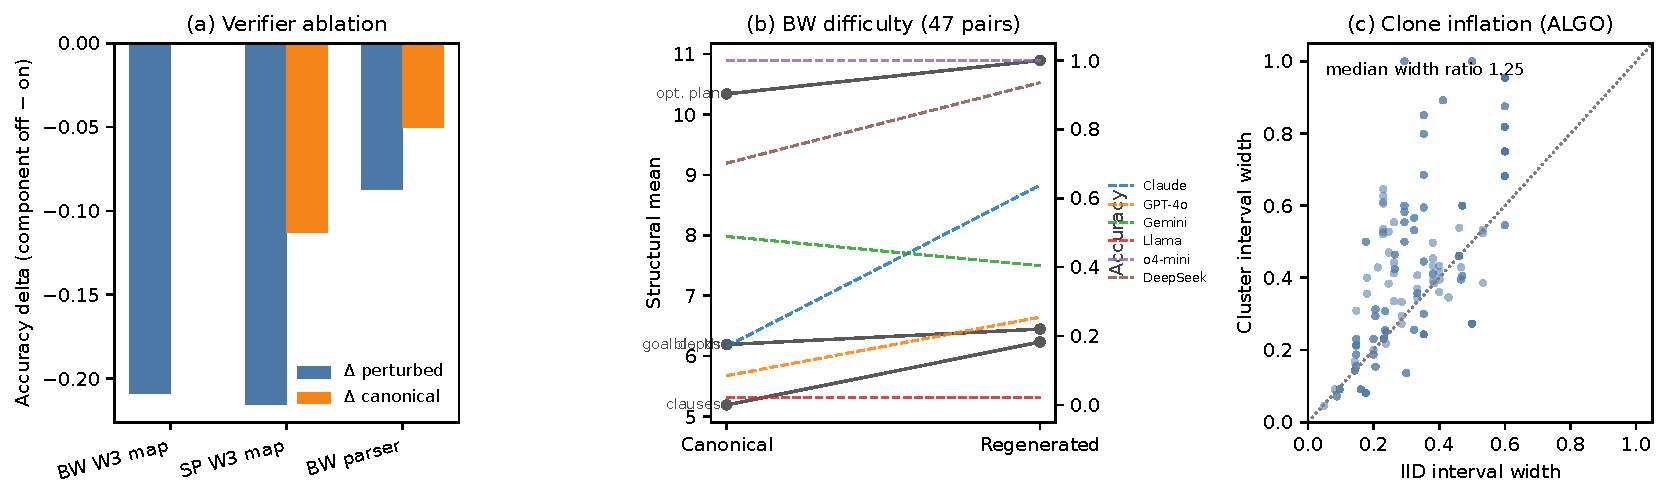
\includegraphics[width=\linewidth]{figures/fig1_confounds.pdf}
\caption{Three confounds that each produce drop-shaped signals. (a)~Oracle repair deltas on
perturbed versus canonical conditions. (b)~Blocksworld structural means (solid) rise under
regeneration while accuracy (dashed) often rises too. (c)~ALGO confidence-interval widths under
iid versus clone-family cluster bootstrap.}
\label{fig:confounds}
\end{figure}

\begin{figure}[t]
\centering
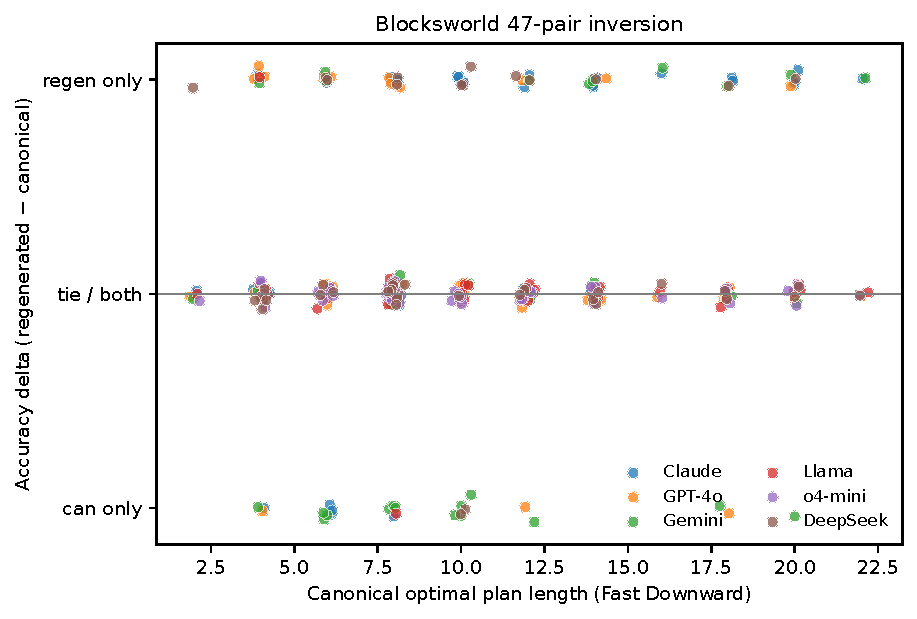
\includegraphics[width=0.85\linewidth]{figures/fig2_bw_inversion.pdf}
\caption{Centrepiece: 47 matched Blocksworld pairs. Each point is one (instance, model) with
canonical optimal plan length on the $x$-axis and regenerated-minus-canonical correctness on the
$y$-axis. Four of six models concentrate above zero despite harder structure.}
\label{fig:bw-inversion}
\end{figure}

\paragraph{Contamination does not account for the gap.} If released instances were harder because
models have memorised them in a way that interferes, per-instance proximity should predict the
canonical-minus-regenerated gap. It does not: Spearman correlations between Infini-gram proximity
and the per-instance gap have intervals spanning zero for five of six models (Claude $-0.14$
$[-0.40, 0.11]$; GPT-4o $-0.11$; Gemini $-0.02$; Llama $-0.18$; DeepSeek $+0.21$). Only o4-mini
shows a significant negative association ($-0.44$ $[-0.60, -0.23]$, $p{=}0.001$).

\paragraph{The effect is domain-specific.} Running the same comparison on the algorithmic family
gives the opposite result: regenerated instances are harder in accuracy for four of five models
(Claude $.667 \rightarrow .244$; o4-mini $1.000 \rightarrow .422$; Gemini $.500 \rightarrow .144$;
GPT-4o $.433 \rightarrow .200$; Llama $.033 \rightarrow .078$), and are structurally mixed rather
than uniformly harder. We therefore do not claim a general property of language models. We claim
that a widely-used planning benchmark's released instances behave differently from instances its
own generator produces, and that any exposure comparison using released items inherits this.

\paragraph{Remaining confounds.}
\textcolor{red}{[PENDING N1 --- do not compile for submission until filled.]}
Two structural variables are not matched by the procedure above. All 50 canonical goals are
single towers, whereas regenerated goals average 1.74 towers; a single tower imposes a strict
construction order that optimal plan length does not capture. Block naming is sequential in 34 of
50 regenerated instances against 5 of 50 canonical. We report the comparison stratified by both
variables in Table~\ref{tab:bw-stratified}. \emph{[Insert stratified result. If the gap survives
both strata, state that. If naming accounts for it, that is the stronger surface-form finding and
this section should be retitled accordingly.]}

\section{Fragility Has No Item-Level Locus}
\label{sec:locus}

Perturbation results are usually reported as marginal accuracies, which implicitly treats
fragility as a property of items: some problems are harder to rename-survive than others. We test
this directly by asking which items fail for \emph{every} model.

\paragraph{No shared-hard set outside obfuscated planning.} Among items where all five models
were evaluated, the number failing for all of them is $0/110$ on the algorithmic family and
$0/20$ on arithmetic. On planning it is $14/64$, and all fourteen are mystery instances. Outside
the obfuscated planning condition, essentially no item is universally fragile. Fragility is a
model--item interaction, not an item property (Figure~\ref{fig:locus}).

\begin{figure}[t]
\centering
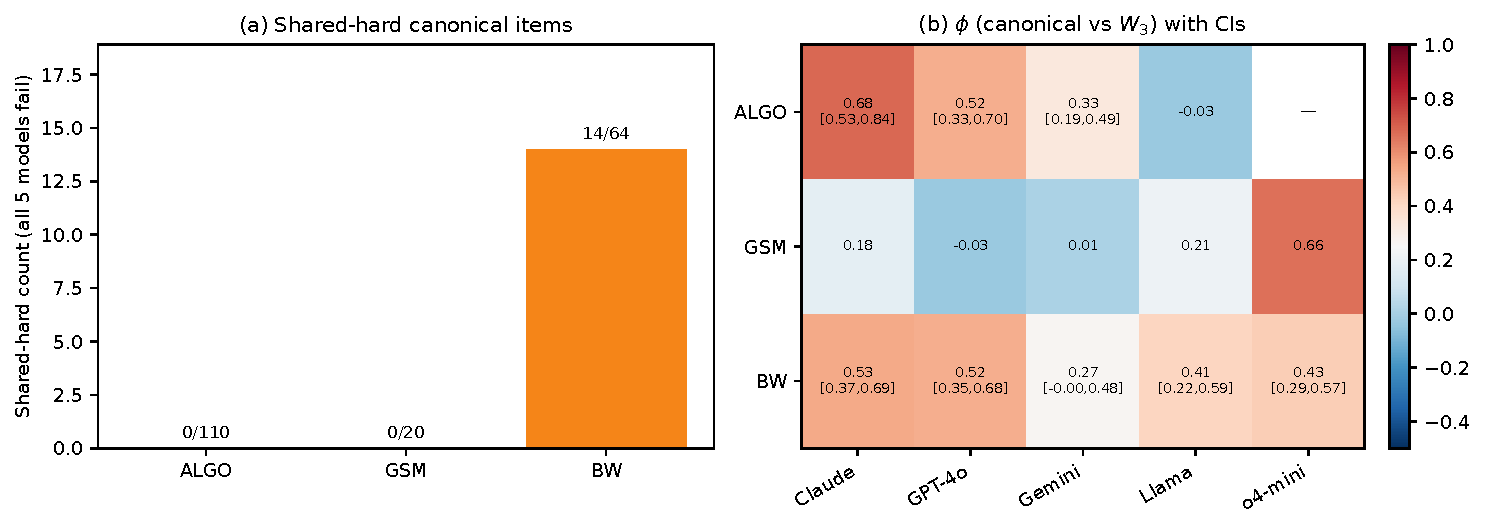
\includegraphics[width=\linewidth]{figures/fig3_locus.pdf}
\caption{Item-level locus. (a)~Shared-hard canonical counts (fail for all five paper models).
(b)~Canonical--$W_3$ contingency coefficient $\phi$ with bootstrap CIs.}
\label{fig:locus}
\end{figure}

\paragraph{Items are not independent.}
\label{sec:clones}
Near-duplicate detection with identical gold answers collapses the 110-problem algorithmic bank
into 14 clone families covering 73 problems, for an effective $n$ of 51; the largest family has
13 members. The frozen 61-item adversarial subset collapses to 14 clusters. Re-estimating
intervals with a cluster bootstrap over families widens them by a median factor of $1.60$ on the
full bank and $1.94$ on the adversarial subset, reaching $2.66$ on individual cells. All ALGO
intervals in this paper use the cluster bootstrap. Because procedural generators produce clone
structure by construction, we expect this to generalise to other generated banks, and we
recommend reporting effective $n$ alongside nominal $n$.

\section{Robustness Is Not a Single Construct}
\label{sec:construct}

If surface invariance and procedural consistency were facets of one underlying robustness
capacity, measures of each should covary. We test this with a measure that is methodologically
independent of the rename probe: a cross-session consistency index (CCI) comparing a model's
declared solution plan, produced in one session, against its step-by-step execution in a second
session with no shared context.

\paragraph{Plan consistency does not predict rename survival.} At the item level, the
point-biserial correlation between CCI and rename survival is $0.156$ $[-0.006, 0.308]$,
$p{=}0.060$, $n{=}128$ (Figure~\ref{fig:construct}); restricted to items the model solves
canonically it is $0.153$, $p{=}0.109$, $n{=}110$. Across models the rank correlation between
mean CCI and retention is $0.600$, $p{=}0.400$, $n{=}4$. The association is consistently positive
and never reaches significance at the sample sizes available. We report this as a null rather
than a trend.

\begin{figure}[t]
\centering
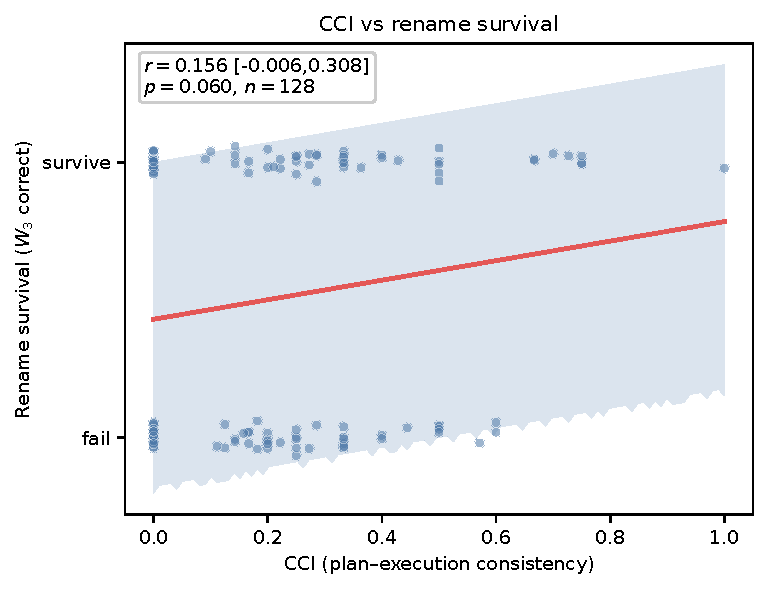
\includegraphics[width=0.72\linewidth]{figures/fig4_construct.pdf}
\caption{CCI versus rename survival on GSM ($n{=}128$), with OLS fit and residual bootstrap band.
Annotated $r$ and $p$ are the cluster-bootstrap point-biserial from
\texttt{P2\_P1\_convergence.csv}.}
\label{fig:construct}
\end{figure}

\paragraph{Discriminant validity.} Neither robustness measure tracks accuracy. Rank correlation
between canonical accuracy and retention is $0.136$ $[-0.100, 0.800]$, $p{=}0.642$; between
canonical accuracy and the canonical--rename contingency coefficient $\phi$ it is $-0.426$
$[-0.724, 0.500]$, $p{=}0.146$. Robustness is measurably distinct from the quantity leaderboards
report. We deliberately do not present retention and $\phi$ as convergent evidence: both are
statistics of the same $2\times 2$ contingency table, so their agreement is algebraic rather than
empirical.

\paragraph{Compliance and correctness are separable.} In a mid-solve injection protocol, models
accept an injected incorrect intermediate state at high rates (Claude 88.5\%, GPT-4o 93.4\%,
o4-mini 100\%, Llama 39.3\%; Gemini treats every injection as malformed input and proceeds
without it) yet post-injection final accuracy stays near uninterrupted rates (Claude .525 vs
.541; GPT-4o .508 vs .557; o4-mini .377 vs .409). Accepting a false premise mid-derivation does
not reliably derail the final answer, so compliance is not a proxy for procedural integrity.

\section{Scope and Planned Work}
\label{sec:scope}

This section states what the present design does not establish and which experiments would
decide each question. Each is specified with the outcome that would confirm or refute it.

\paragraph{Instrument boundaries.} Two measurement limits are themselves findings rather than
gaps. Under a strict PDDL execution protocol, 84--100\% of planning sessions abort on illegal
actions; routing through a natural-language tolerant parser shifts the failure mode from format
errors (1729 to 451) to precondition violations (258 to 1469), which establishes that models
emit genuinely illegal plans rather than mis-formatted valid ones. Given canonical planning
accuracy of .02--.22 for three of the models, plan-execution coupling is undefined at that floor.
Separately, planning gold answers use three distinct first-action tokens across 65 problems, so
rank-based readouts over the gold token cannot discriminate conditions in that family. Both are
scope conditions on the method, not failures of it.

\paragraph{Underdetermined convergence rules.} We implemented a per-instance label combining all
three probes through a five-parameter conjunction. Across a 270-configuration threshold sweep the
retrieval-consistent count ranges from 0 to 170 of 440 instances. With five free parameters and
this sample size the labelling is underdetermined, and we therefore report probe-level results
rather than per-instance labels. Constraining the rule requires ground-truth exposure labels,
which are available only for open-weight models with published corpora; a calibration study on
such a model is the next step, with the pre-registered criterion that labels track known exposure
at AUC $\ge 0.75$.

\paragraph{Queued measurements.} The following are specified and blocked on inference budget
rather than design. \emph{(i)} Direction-reversal on the graph family: prompts are regenerated
and gold verified under Bellman--Ford, awaiting a 250-call sweep; the design predicts a floor
effect distinguishing reversal from rename. \emph{(ii)} Phase-resolved execution accuracy on
arithmetic: the current implementation pools two sessions, so we report consistency and error
propagation but not phase-resolved accuracy; a 220-session re-run persisting per-step values
would resolve it. \emph{(iii)} A difficulty-matched weighted-interval bank, since exposure and
difficulty covary in the present design and cannot be separated.

\paragraph{Mechanistic follow-up.} We ran a single-backbone logit-lens pilot reading gold-token
rank through the residual stream. It is a pilot in the strict sense: one open-weight model, and
quantisation differs across the backbones we compared, so cross-model contrasts are confounded.
The planning-family degeneracy noted above further bounds what the readout can measure there.
A multi-backbone unquantised replication is the immediate next experiment; the prediction under
a representational account is that rename-induced shift in gold-token accessibility should
predict per-item rename survival within a model.

\paragraph{Programme.} These sit within a staged programme: establishing and validating the
instrument (this work), locating the behavioural dissociation representationally, characterising
the training-data conditions under which invariance forms, and tracking its emergence across
public checkpoint series. Instrument validation is the precondition for all three, which is why
we report it as a result rather than as an appendix.

\section{Conclusion}

Perturbation benchmarks measure a real phenomenon, but the protocol as commonly implemented
conflates it with at least three others. The answer-checker fails in a manner correlated with the
treatment and biased toward the hypothesis. Regenerated and released instances differ in
difficulty, and on a widely-used planning benchmark the released instances are the harder ones to
solve despite being structurally easier. Generated banks contain clone families that halve the
effective sample size. Once these are handled, fragility turns out to have no item-level locus
outside obfuscated planning, and procedural consistency does not predict surface invariance ---
so robustness is not one thing, and reporting it as one number reproduces the problem that
motivated perturbation testing in the first place.

\bibliographystyle{plainnat}
\bibliography{references}

\appendix

\section{Variant Generation Protocol}
\label{app:variants}

\textbf{W1 (paraphrase).} Restated in different words; numeric values, entities, and structural
relations preserved exactly.
\textbf{W2 (format).} Prose converted to a structured representation appropriate to the family
(adjacency matrix, interval table, equation set).
\textbf{W3 (entity rename).} All entity identifiers replaced with a held-out,
vocabulary-disjoint token set, length-matched and single-token where the original was
single-token. The generator persists the mapping; the verifier consumes it
(Section~\ref{sec:oracle}).
\textbf{W4 (formal notation).} \LaTeX{} for arithmetic, formal predicates for planning,
mathematical edge-list notation for graph and interval problems.
\textbf{W5 (direction reversal).} Planning: initial and goal states exchanged. Arithmetic:
forward problems inverted to backward form. Graph: source and destination exchanged. Not defined
for coin change or interval scheduling, which have no meaningful reversal.
\textbf{W6 (procedural regeneration).} Same algorithm and parameter ranges, new numeric values.
A regenerated item is retained only if its gold answer differs from the canonical and its text is
not byte-identical.

Every variant passes its family verifier on the gold answer before any model is queried.

\section{Coverage and Exclusions}
\label{app:coverage}

\begin{table}[t]
  \centering
  \scriptsize
  \setlength{\tabcolsep}{2.5pt}
  \caption{Coverage and exclusions from \texttt{COVERAGE\_MASTER.csv}.
  One row per (probe, family, model, variant).}
  \label{tab:coverage}
  \begin{tabular}{llllrrrl}
    \toprule
    Probe & Family & Model & Variant & Att. & Incl. & Excl. & Top exclusion \\
    \midrule
    P1 & ALGO & Claude & W1 & 110 & 110 & 0 & --- \\
    P1 & ALGO & Claude & W2 & 110 & 110 & 0 & --- \\
    P1 & ALGO & Claude & W3 & 110 & 100 & 10 & parse\_failed \\
    P1 & ALGO & Claude & W4 & 110 & 108 & 2 & parse\_failed \\
    P1 & ALGO & Claude & W5 & 50 & 50 & 0 & --- \\
    P1 & ALGO & Claude & W6 & 90 & 90 & 0 & --- \\
    P1 & ALGO & Claude & canonical & 110 & 110 & 0 & --- \\
    P1 & ALGO & Gemini & W1 & 110 & 110 & 0 & --- \\
    P1 & ALGO & Gemini & W2 & 110 & 110 & 0 & --- \\
    P1 & ALGO & Gemini & W3 & 110 & 105 & 5 & parse\_failed \\
    P1 & ALGO & Gemini & W4 & 110 & 105 & 5 & parse\_failed \\
    P1 & ALGO & Gemini & W5 & 50 & 32 & 18 & parse\_failed \\
    P1 & ALGO & Gemini & W6 & 90 & 86 & 4 & parse\_failed \\
    P1 & ALGO & Gemini & canonical & 110 & 110 & 0 & --- \\
    P1 & ALGO & Llama & W1 & 110 & 110 & 0 & --- \\
    P1 & ALGO & Llama & W2 & 110 & 104 & 6 & parse\_failed \\
    P1 & ALGO & Llama & W3 & 110 & 109 & 1 & parse\_failed \\
    P1 & ALGO & Llama & W4 & 110 & 106 & 4 & parse\_failed \\
    P1 & ALGO & Llama & W5 & 50 & 50 & 0 & --- \\
    P1 & ALGO & Llama & W6 & 110 & 90 & 20 & missing\_bank\_row \\
    P1 & ALGO & Llama & canonical & 110 & 110 & 0 & --- \\
    P1 & ALGO & mock & W1 & 1 & 0 & 1 & mock\_row \\
    P1 & ALGO & mock & W1 & 1 & 0 & 1 & mock\_row \\
    P1 & ALGO & mock & W2 & 1 & 0 & 1 & mock\_row \\
    P1 & ALGO & mock & canonical & 1 & 0 & 1 & mock\_row \\
    P1 & ALGO & mock & canonical & 1 & 0 & 1 & mock\_row \\
    P1 & ALGO & GPT-4o & W1 & 110 & 110 & 0 & --- \\
    P1 & ALGO & GPT-4o & W2 & 110 & 110 & 0 & --- \\
    P1 & ALGO & GPT-4o & W3 & 110 & 102 & 8 & parse\_failed \\
    P1 & ALGO & GPT-4o & W4 & 110 & 110 & 0 & --- \\
    P1 & ALGO & GPT-4o & W5 & 50 & 22 & 28 & parse\_failed \\
    P1 & ALGO & GPT-4o & W6 & 110 & 90 & 20 & missing\_bank\_row \\
    P1 & ALGO & GPT-4o & canonical & 110 & 110 & 0 & --- \\
    P1 & ALGO & o4-mini & W1 & 110 & 109 & 1 & parse\_failed \\
    P1 & ALGO & o4-mini & W2 & 110 & 105 & 5 & parse\_failed \\
    P1 & ALGO & o4-mini & W3 & 110 & 81 & 29 & parse\_failed \\
    P1 & ALGO & o4-mini & W4 & 110 & 97 & 13 & parse\_failed \\
    P1 & ALGO & o4-mini & W5 & 50 & 8 & 42 & parse\_failed \\
    P1 & ALGO & o4-mini & W6 & 90 & 89 & 1 & parse\_failed \\
    P1 & ALGO & o4-mini & canonical & 110 & 110 & 0 & --- \\
    P1 & BW & The answer is 42. & MOCK & 4 & 0 & 4 & mock\_row \\
    P1 & BW & Claude & W1 & 109 & 102 & 7 & invalid\_gold \\
    P1 & BW & Claude & W2 & 109 & 103 & 6 & invalid\_gold \\
    P1 & BW & Claude & W3 & 109 & 104 & 5 & invalid\_gold \\
    P1 & BW & Claude & W4 & 109 & 103 & 6 & invalid\_gold \\
    P1 & BW & Claude & W5 & 109 & 99 & 10 & invalid\_gold \\
    P1 & BW & Claude & W6 & 89 & 84 & 5 & invalid\_gold \\
    P1 & BW & Claude & canonical & 109 & 108 & 1 & invalid\_gold \\
    P1 & BW & DeepSeek & W1 & 65 & 58 & 7 & invalid\_gold \\
    P1 & BW & DeepSeek & W2 & 65 & 59 & 6 & invalid\_gold \\
    P1 & BW & DeepSeek & W3 & 65 & 60 & 5 & invalid\_gold \\
    P1 & BW & DeepSeek & W4 & 65 & 59 & 6 & invalid\_gold \\
    P1 & BW & DeepSeek & W5 & 65 & 55 & 10 & invalid\_gold \\
    P1 & BW & DeepSeek & W6 & 65 & 60 & 5 & invalid\_gold \\
    P1 & BW & DeepSeek & canonical & 49 & 48 & 1 & invalid\_gold \\
    P1 & BW & Gemini & W1 & 65 & 58 & 7 & invalid\_gold \\
    P1 & BW & Gemini & W2 & 65 & 59 & 6 & invalid\_gold \\
    P1 & BW & Gemini & W3 & 65 & 60 & 5 & invalid\_gold \\
    P1 & BW & Gemini & W4 & 65 & 59 & 6 & invalid\_gold \\
    P1 & BW & Gemini & W5 & 65 & 55 & 10 & invalid\_gold \\
    P1 & BW & Gemini & W6 & 65 & 60 & 5 & invalid\_gold \\
    P1 & BW & Gemini & canonical & 65 & 64 & 1 & invalid\_gold \\
    P1 & BW & Llama & W1 & 109 & 102 & 7 & invalid\_gold \\
    P1 & BW & Llama & W2 & 109 & 103 & 6 & invalid\_gold \\
    P1 & BW & Llama & W3 & 109 & 103 & 6 & invalid\_gold \\
    P1 & BW & Llama & W4 & 109 & 102 & 7 & invalid\_gold \\
    P1 & BW & Llama & W5 & 109 & 99 & 10 & invalid\_gold \\
    P1 & BW & Llama & W6 & 104 & 84 & 20 & missing\_bank\_row \\
    P1 & BW & Llama & canonical & 109 & 108 & 1 & invalid\_gold \\
    P1 & BW & mock & W1 & 1 & 0 & 1 & mock\_row \\
    P1 & BW & mock & W2 & 11 & 0 & 11 & mock\_row \\
    P1 & BW & mock & W3 & 10 & 0 & 10 & mock\_row \\
    P1 & BW & mock & W4 & 10 & 0 & 10 & mock\_row \\
    P1 & BW & mock & W5 & 9 & 0 & 9 & mock\_row \\
    P1 & BW & mock & canonical & 17 & 0 & 17 & mock\_row \\
    P1 & BW & GPT-4o & W1 & 109 & 102 & 7 & invalid\_gold \\
    P1 & BW & GPT-4o & W2 & 109 & 103 & 6 & invalid\_gold \\
    P1 & BW & GPT-4o & W3 & 109 & 104 & 5 & invalid\_gold \\
    P1 & BW & GPT-4o & W4 & 109 & 103 & 6 & invalid\_gold \\
    P1 & BW & GPT-4o & W5 & 109 & 99 & 10 & invalid\_gold \\
    P1 & BW & GPT-4o & W6 & 104 & 84 & 20 & missing\_bank\_row \\
    P1 & BW & GPT-4o & canonical & 109 & 108 & 1 & invalid\_gold \\
    P1 & BW & o4-mini & W1 & 65 & 58 & 7 & invalid\_gold \\
    P1 & BW & o4-mini & W2 & 65 & 59 & 6 & invalid\_gold \\
    P1 & BW & o4-mini & W3 & 65 & 60 & 5 & invalid\_gold \\
    P1 & BW & o4-mini & W4 & 65 & 59 & 6 & invalid\_gold \\
    P1 & BW & o4-mini & W5 & 65 & 55 & 10 & invalid\_gold \\
    P1 & BW & o4-mini & W6 & 65 & 60 & 5 & invalid\_gold \\
    P1 & BW & o4-mini & canonical & 65 & 64 & 1 & invalid\_gold \\
    P1 & GSM & Claude & W1 & 44 & 44 & 0 & --- \\
    P1 & GSM & Claude & W2 & 44 & 44 & 0 & --- \\
    P1 & GSM & Claude & W3 & 44 & 44 & 0 & --- \\
    P1 & GSM & Claude & W4 & 44 & 44 & 0 & --- \\
    P1 & GSM & Claude & W5 & 44 & 44 & 0 & --- \\
    P1 & GSM & Claude & W6 & 24 & 24 & 0 & --- \\
    P1 & GSM & Claude & canonical & 44 & 44 & 0 & --- \\
    P1 & GSM & Gemini & W1 & 44 & 44 & 0 & --- \\
    P1 & GSM & Gemini & W2 & 44 & 44 & 0 & --- \\
    P1 & GSM & Gemini & W3 & 44 & 44 & 0 & --- \\
    P1 & GSM & Gemini & W4 & 44 & 44 & 0 & --- \\
    P1 & GSM & Gemini & W5 & 44 & 44 & 0 & --- \\
    P1 & GSM & Gemini & W6 & 24 & 24 & 0 & --- \\
    P1 & GSM & Gemini & canonical & 44 & 44 & 0 & --- \\
    P1 & GSM & Llama & W1 & 64 & 20 & 44 & api\_error \\
    P1 & GSM & Llama & W2 & 64 & 20 & 44 & api\_error \\
    P1 & GSM & Llama & W3 & 64 & 20 & 44 & api\_error \\
    P1 & GSM & Llama & W4 & 64 & 20 & 44 & api\_error \\
    P1 & GSM & Llama & W5 & 64 & 20 & 44 & api\_error \\
    P1 & GSM & Llama & W6 & 64 & 0 & 64 & missing\_bank\_row \\
    P1 & GSM & Llama & canonical & 64 & 20 & 44 & api\_error \\
    P1 & GSM & GPT-4o & W1 & 64 & 20 & 44 & api\_error \\
    P1 & GSM & GPT-4o & W2 & 64 & 20 & 44 & api\_error \\
    P1 & GSM & GPT-4o & W3 & 64 & 20 & 44 & api\_error \\
    P1 & GSM & GPT-4o & W4 & 64 & 20 & 44 & api\_error \\
    P1 & GSM & GPT-4o & W5 & 64 & 20 & 44 & api\_error \\
    P1 & GSM & GPT-4o & W6 & 64 & 0 & 64 & missing\_bank\_row \\
    P1 & GSM & GPT-4o & canonical & 64 & 20 & 44 & api\_error \\
    P1 & GSM & o4-mini & W1 & 44 & 44 & 0 & --- \\
    P1 & GSM & o4-mini & W2 & 44 & 44 & 0 & --- \\
    P1 & GSM & o4-mini & W3 & 44 & 44 & 0 & --- \\
    P1 & GSM & o4-mini & W4 & 44 & 44 & 0 & --- \\
    P1 & GSM & o4-mini & W5 & 44 & 44 & 0 & --- \\
    P1 & GSM & o4-mini & W6 & 24 & 24 & 0 & --- \\
    P1 & GSM & o4-mini & canonical & 44 & 44 & 0 & --- \\
    P2 & ALGO & Claude & phase1 & 110 & 84 & 26 & phase1\_unparseable \\
    P2 & ALGO & Gemini & phase1 & 110 & 72 & 38 & phase1\_unparseable \\
    P2 & ALGO & Llama & phase1 & 110 & 76 & 34 & phase1\_unparseable \\
    P2 & ALGO & GPT-4o & phase1 & 110 & 94 & 16 & phase1\_unparseable \\
    P2 & BW & Claude & cci\_nl & 50 & 20 & 30 & aborted: excessive illegal steps \\
    P2 & BW & Claude & cci\_strict & 50 & 8 & 42 & aborted: excessive illegal steps \\
    P2 & BW & Claude & tep & 177 & 1 & 176 & aborted: excessive illegal steps \\
    P2 & BW & Llama & cci\_nl & 50 & 8 & 42 & aborted: excessive illegal steps \\
    P2 & BW & Llama & cci\_strict & 50 & 11 & 39 & blank\_session\_status \\
    P2 & BW & Llama & tep & 179 & 0 & 179 & blank\_session\_status \\
    P2 & BW & GPT-4o & cci\_nl & 50 & 11 & 39 & aborted: excessive illegal steps \\
    P2 & BW & GPT-4o & cci\_strict & 50 & 10 & 40 & blank\_session\_status \\
    P2 & BW & GPT-4o & tep & 180 & 1 & 179 & blank\_session\_status \\
    P2 & GSM & Claude & cci & 44 & 44 & 0 & --- \\
    P2 & GSM & Claude & tep & 44 & 44 & 0 & --- \\
    P2 & GSM & Gemini & cci & 44 & 44 & 0 & --- \\
    P2 & GSM & Gemini & tep & 44 & 44 & 0 & --- \\
    P2 & GSM & Llama & cci & 44 & 44 & 0 & --- \\
    P2 & GSM & Llama & tep & 44 & 44 & 0 & --- \\
    P2 & GSM & GPT-4o & cci & 44 & 44 & 0 & --- \\
    P2 & GSM & GPT-4o & tep & 44 & 44 & 0 & --- \\
    P2 & MBW & Claude & cci\_nl & 15 & 0 & 15 & cci\_column\_never\_emitted \\
    P2 & MBW & Llama & cci\_nl & 15 & 0 & 15 & cci\_column\_never\_emitted \\
    P2 & MBW & GPT-4o & cci\_nl & 15 & 0 & 15 & cci\_column\_never\_emitted \\
    P3 & ALGO & -- & contamination & 116 & 116 & 0 & --- \\
    P3 & ALGO & Qwen2.5-0.5B-Instr & canonical & 20 & 20 & 0 & --- \\
    P3 & BW & -- & contamination & 65 & 65 & 0 & --- \\
    P3 & BW & Qwen2.5-0.5B-Instr & W6 & 15 & 15 & 0 & --- \\
    P3 & BW & Qwen2.5-0.5B-Instr & canonical & 20 & 20 & 0 & --- \\
    P3 & GSM & -- & contamination & 44 & 44 & 0 & --- \\
    P3 & GSM & Qwen2.5-0.5B-Instr & canonical & 20 & 20 & 0 & --- \\
    \bottomrule
  \end{tabular}
\end{table}


Full per-(family, slice, model, variant) Probe~1 accuracies with CIs are in
Table~\ref{tab:variants} (\texttt{tables/table\_variants.tex}), regenerated from rescored
\texttt{included=True} rows consistent with \texttt{P1\_rescore\_summary.csv}.

\begin{table}[t]
  \centering
  \scriptsize
  \setlength{\tabcolsep}{3pt}
  \caption{Per-variant accuracy by family, slice, and model (Probe~1).
  Accuracies use rescored \texttt{included=True} rows consistent with
  \texttt{results/derived/P1\_rescore\_summary.csv}. ALGO intervals are
  10k cluster-bootstrap CIs over clone families (seed~42); GSM/BW use
  Wilson 95\% CIs. Excluded cells show the exclusion reason, never 0.}
  \label{tab:variants}
  \begin{tabular}{lllccccccc}
    \toprule
    Family & Slice & Model & Can. & W1 & W2 & W3 & W4 & W5 & W6 \\
    \midrule
    GSM & -- & Claude     & .841 [.71,.92] & .841 [.71,.92] & .773 [.63,.87] & .750 [.61,.85] & .636 [.49,.76] & .818 [.68,.90] & .750 [.55,.88] \\
    GSM & -- & GPT-4o     & .850 [.64,.95] & .750 [.53,.89] & .300 [.15,.52] & .300 [.15,.52] & .200 [.08,.42] & .300 [.15,.52] & \textit{missing\_bank\_row} \\
    GSM & -- & Gemini     & .909 [.79,.96] & .818 [.68,.90] & .636 [.49,.76] & .523 [.38,.66] & .477 [.34,.62] & .614 [.47,.74] & .958 [.80,.99] \\
    GSM & -- & Llama      & .800 [.58,.92] & .850 [.64,.95] & .250 [.11,.47] & .150 [.05,.36] & .300 [.15,.52] & .050 [.01,.24] & \textit{missing\_bank\_row} \\
    GSM & -- & \omini     & .841 [.71,.92] & .864 [.73,.94] & .818 [.68,.90] & .841 [.71,.92] & .682 [.53,.80] & .886 [.76,.95] & .833 [.64,.93] \\
    \midrule
    ALGO & CC-chall & Claude     & .700 [.00,.95] & .700 [.00,.88] & .700 [.00,.95] & .600 [.00,.75] & .800 [.00,1.00] & \textit{not defined} & \textit{variant\_not\_transformed} \\
    ALGO & CC-chall & GPT-4o     & .600 [.00,.75] & .400 [.00,.55] & .600 [.00,.82] & .600 [.00,.82] & .500 [.00,.68] & \textit{not defined} & \textit{missing\_bank\_row} \\
    ALGO & CC-chall & Gemini     & .500 [.00,.68] & .700 [.00,.95] & .600 [.00,.82] & .700 [.00,.95] & .700 [.00,.95] & \textit{not defined} & \textit{variant\_not\_transformed} \\
    ALGO & CC-chall & Llama      & .200 [.00,.27] & .100 [.00,.14] & .400 [.00,.75] & .000 [.00,.00] & .222 [.00,.32] & \textit{not defined} & \textit{missing\_bank\_row} \\
    ALGO & CC-std & Claude     & .267 [.07,.47] & .467 [.20,.73] & .067 [.00,.23] & .300 [.00,.56] & .667 [.44,.87] & \textit{not defined} & .067 [.00,.23] \\
    ALGO & CC-std & GPT-4o     & .267 [.08,.44] & .400 [.21,.60] & .000 [.00,.00] & .071 [.00,.20] & .867 [.64,1.00] & \textit{not defined} & .200 [.00,.43] \\
    ALGO & CC-std & Gemini     & .267 [.07,.47] & .133 [.00,.36] & .000 [.00,.00] & .000 [.00,.00] & .267 [.07,.47] & \textit{not defined} & .267 [.07,.50] \\
    ALGO & CC-std & Llama      & .000 [.00,.00] & .067 [.00,.23] & .111 [.00,.30] & .000 [.00,.00] & .000 [.00,.00] & \textit{not defined} & .067 [.00,.23] \\
    ALGO & SP-chall & Claude     & .941 [.69,1.00] & .941 [.81,1.00] & .676 [.35,.92] & .882 [.63,.98] & .941 [.69,1.00] & .000 [.00,.00] & .323 [.25,.36] \\
    ALGO & SP-chall & GPT-4o     & .412 [.04,.89] & .529 [.29,.89] & .147 [.00,.26] & .294 [.04,.69] & .676 [.24,.95] & .000 [.00,.00] & .258 [.25,.27] \\
    ALGO & SP-chall & Gemini     & .706 [.41,.93] & .471 [.11,.77] & .235 [.04,.50] & .353 [.15,.78] & .912 [.77,.97] & .100 [.00,.25] & .129 [.00,.18] \\
    ALGO & SP-chall & Llama      & .029 [.00,.10] & .147 [.00,.31] & .029 [.00,.07] & .000 [.00,.00] & .088 [.00,.15] & .000 [.00,.00] & .129 [.00,.25] \\
    ALGO & SP-std & Claude     & .952 [.83,1.00] & 1.000 [1.00,1.00] & .762 [.54,.95] & 1.000 [1.00,1.00] & 1.000 [1.00,1.00] & .053 [.00,.16] & .579 [.33,.80] \\
    ALGO & SP-std & GPT-4o     & .762 [.54,.95] & .667 [.44,.86] & .048 [.00,.14] & .476 [.29,.67] & .714 [.50,.89] & .000 [.00,.00] & .368 [.11,.63] \\
    ALGO & SP-std & Gemini     & .619 [.41,.82] & .762 [.57,.92] & .810 [.60,1.00] & .476 [.22,.71] & 1.000 [1.00,1.00] & .083 [.00,.23] & .333 [.00,.65] \\
    ALGO & SP-std & Llama      & .048 [.00,.14] & .143 [.00,.27] & .000 [.00,.00] & .000 [.00,.00] & .143 [.00,.29] & .053 [.00,.16] & .105 [.00,.24] \\
    ALGO & WIS-chall & Claude     & .353 [.00,.60] & .176 [.00,.30] & .118 [.00,.50] & .000 [.00,.00] & .067 [.00,.60] & \textit{not defined} & \textit{variant\_not\_transformed} \\
    ALGO & WIS-chall & GPT-4o     & .353 [.00,.41] & .176 [.00,.24] & .000 [.00,.00] & .000 [.00,.00] & .000 [.00,.00] & \textit{not defined} & \textit{no included} \\
    ALGO & WIS-chall & Gemini     & .353 [.00,.60] & .176 [.00,.24] & .000 [.00,.00] & .000 [.00,.00] & .000 [.00,.00] & \textit{not defined} & \textit{variant\_not\_transformed} \\
    ALGO & WIS-chall & Llama      & .059 [.00,.08] & .000 [.00,.00] & .000 [.00,.00] & .059 [.00,.08] & .000 [.00,.00] & \textit{not defined} & \textit{no included} \\
    ALGO & WIS-std & Claude     & .077 [.00,.23] & .231 [.00,.46] & .231 [.00,.46] & .091 [.00,.27] & .077 [.00,.23] & \textit{not defined} & \textit{variant\_not\_transformed} \\
    ALGO & WIS-std & GPT-4o     & .154 [.00,.38] & .231 [.00,.46] & .000 [.00,.00] & .000 [.00,.00] & .000 [.00,.00] & \textit{not defined} & \textit{no included} \\
    ALGO & WIS-std & Gemini     & .000 [.00,.00] & .000 [.00,.00] & .231 [.00,.46] & .182 [.00,.45] & .000 [.00,.00] & \textit{not defined} & \textit{variant\_not\_transformed} \\
    ALGO & WIS-std & Llama      & .000 [.00,.00] & .000 [.00,.00] & .000 [.00,.00] & .077 [.00,.23] & .000 [.00,.00] & \textit{not defined} & \textit{no included} \\
    \midrule
    BW & -- & Claude     & .172 [.10,.28] & .138 [.07,.25] & .305 [.20,.43] & .100 [.05,.20] & .119 [.06,.23] & .873 [.76,.94] & .673 [.54,.78] \\
    BW & -- & GPT-4o     & .063 [.02,.15] & .172 [.10,.29] & .102 [.05,.20] & .100 [.05,.20] & .119 [.06,.23] & .291 [.19,.42] & .250 [.15,.38] \\
    BW & -- & Gemini     & .391 [.28,.51] & .259 [.16,.38] & .237 [.15,.36] & .133 [.07,.24] & .068 [.03,.16] & .764 [.64,.86] & .404 [.28,.54] \\
    BW & -- & Llama      & .016 [.00,.08] & .052 [.02,.14] & .017 [.00,.09] & .050 [.02,.14] & .000 [.00,.06] & .000 [.00,.07] & .019 [.00,.10] \\
    BW & -- & \omini     & .781 [.67,.86] & .862 [.75,.93] & .831 [.72,.91] & .483 [.36,.61] & .475 [.35,.60] & .909 [.80,.96] & 1.000 [.93,1.00] \\
    \bottomrule
  \end{tabular}
\end{table}


\section{Metric Definitions}
\label{app:metrics}

$R_{W3} = \mathrm{Acc}_{W3}/\mathrm{Acc}_{\mathrm{can}}$, reported only where
$\mathrm{Acc}_{\mathrm{can}} \ge 0.30$.
$\phi$ is the contingency coefficient of canonical and rename correctness over items.
CCI is the fraction of declared numeric steps matched by second-session execution within
$\epsilon{=}0.01$.
Error propagation is the fraction of post-injection steps differing from the uninjected run.
Proximity is Infini-gram $n$-gram overlap against public corpora, used only within family;
window sizes differ across families (maximum $n{=}8$ for arithmetic, $13$ for the others) and the
count is unnormalised, so cross-family comparison is not valid.

\end{document}
